
\section{Evaluation Results}
\label{sec:eva}

Three experiments evaluate \name{}'s graph coverage,
answer accuracy, and source of effectiveness. Then we visualize the
\abr{gnn} attention and examine individual examples.


\begin{figure*}[t]
\centering
\small
 \begin{subfigure}{0.3\textwidth}
        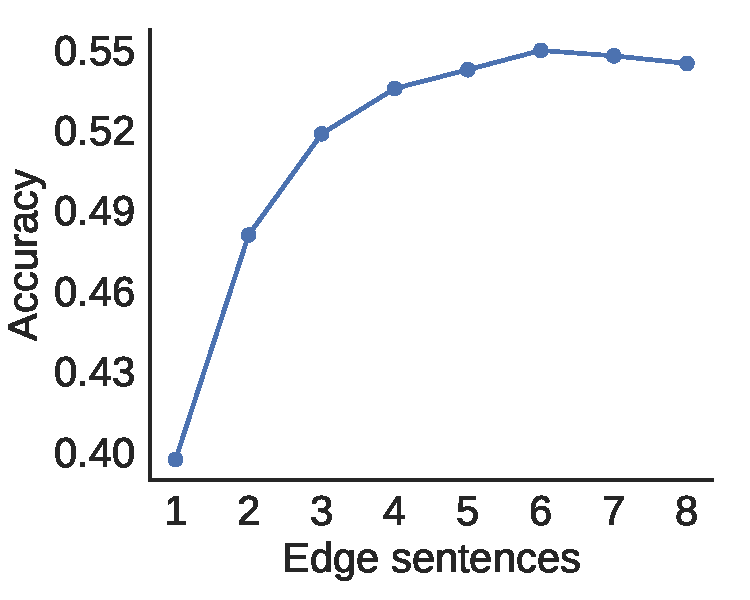
\includegraphics[width=\textwidth]{2020_www_delft/figures/EdgeAccu.pdf}
        \centering
        \caption{Number of Edge Sentences}
    \end{subfigure}
   \begin{subfigure}{0.3\textwidth}
        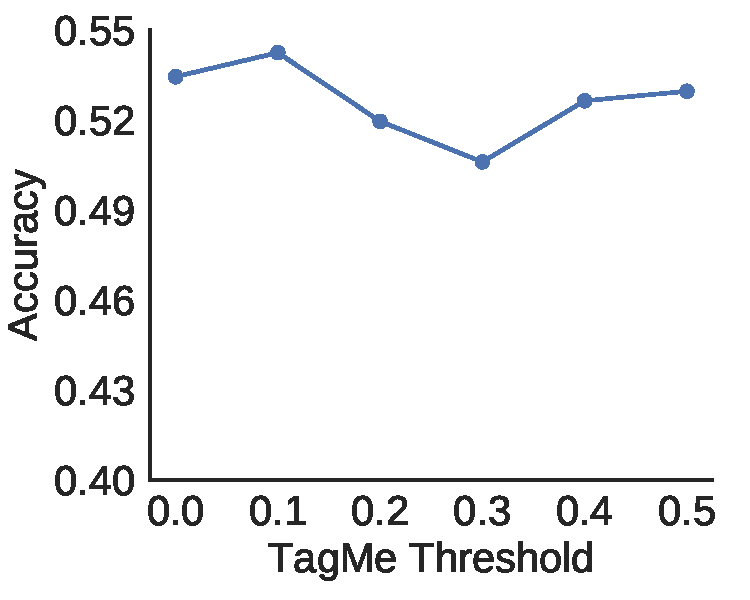
\includegraphics[width=\textwidth]{2020_www_delft/figures/TagmeAccu.pdf}
        \centering
        \caption{TagMe Threshold on Question Entities}
    \end{subfigure}
    \begin{subfigure}{0.3\textwidth}
        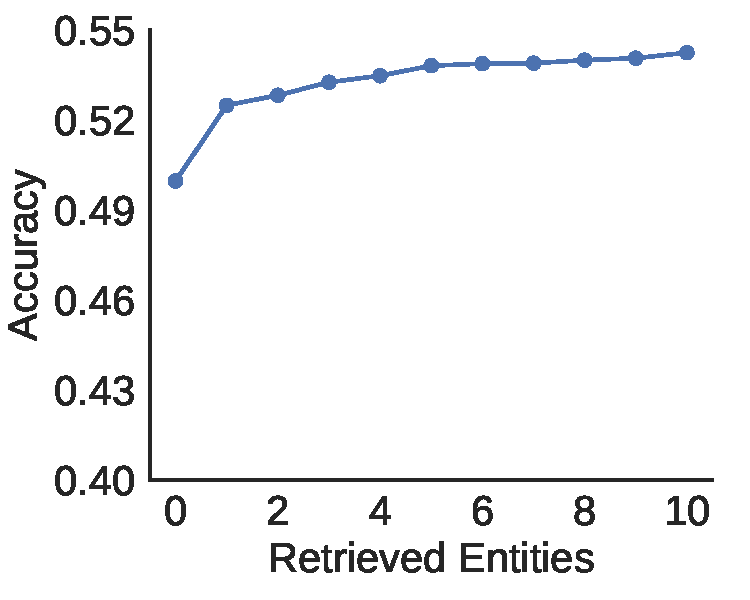
\includegraphics[width=\textwidth]{2020_www_delft/figures/ESAccu.pdf}
        \centering
        \caption{Number of Retrieved Entities}
    \end{subfigure}
\caption{Accuracy of \name{} on different variations of Free-Text Knowledge Graphs.
\label{fig:analysis}
}
\end{figure*}

\subsection{Graph Coverage}
\label{sec:coverage}

\name{}'s graph has high coverage (Table~\ref{tab:coverage}).  
Each question is connected to an average of 1500+ candidate nodes; 90\%
of them can be answered by the connected nodes.
%
After filtering to $50$ candidates, more than 80\% questions are
answerable.
%
In comparison, we manually examined 50 randomly sampled \qblink{}
questions: only 38\% of them are reachable within two hops in the
DBpedia graph.

\name{}'s graph is dense.
%
On average there are five (\qblink{}) and twelve (\qanta{}) edges connecting the
correct answer nodes to the question entity nodes.
%
\triviaqa{} questions have two entities on average and more than one
is connected to the correct answer.  Each edge has eight to fifteen
evidence sentences.

The free-text knowledge graph naturally separates the correct answer by its structure.
%
Compared to incorrect answers (-), the correct ones (+) are connected by significantly more evidence edges.
%
The edges also have more evidence sentences.

Aided by free-text evidence, the coverage of the structured graph is
no longer the bottleneck.
%
The free-text knowledge graph provides enough evidence and frees the
potential of structured ~\abr{qa}.
%
At the same time, the rich evidence also inevitably introduces noise.
%
The next experiment examines whether \name{}---given the answer
somewhere in the graph---can find the single correct answer.

%\czcomment{re-word this sentence}



\begin{table}[t]
  \centering
  \small
  \begin{tabular}{lrr}
    \textbf{Ablation}  & \multicolumn{2}{r}{\textbf{Accuracy}} \\ \toprule
    No Node Pruning & 42.6 & -21.4\% \\ 
    No Gloss Representation & 49.2 & -9.3\% \\ 
    No Edge Evidence Sentence & 48.8 & -10.0\% \\ 
    No Edge Importance & 52.6 & -3.0\% \\ 
    No Self Attention Layer & 53.0 & -2.2\% \\ 
    \name{}-\glove{} &54.2 & -- \\
    \bottomrule
  \end{tabular}
  \caption{Ablation Study of \name{}-\abr{g}{\small love} on \qblink{} (ALL questions). 
    Each \name{} variant removes one component and keeps everything else fixed. }
    \label{tab:ablation} 
\end{table}


\subsection{Answer Accuracy}
% lists the answer accuracy of \name{} and baselines. 
% on ALL questions anddifferent number of entities in the question.
\name{} outperforms\footnote{Recall, however, that we exclude
  questions that with no entities or whose answer is not an entity.}
all baselines on both full datasets and dataset subsets based on the
number of entities in a question (Table~\ref{tab:results}).

\quest{} falters on these questions, suggesting that some level of
supervision is required.
%
On more complicated factoid \abr{qa} datasets \qblink{} and \qanta{},
\name{} improves over \drqa{}, 
the machine reading  baseline.
%
These datasets require reasoning over multiple sentences (either
within a long question's sentence or across multiple questions); however,
\drqa{} is tuned for single sentence questions.
%
\name{}---by design---focuses on matching questions' text with
disparate evidence.
%
In the \abr{mr} benchmark dataset \triviaqa{}, \name{} still beats
\drqa{} (albeit on an entity-focused subset).
%
It is also better than \docqa{}, one of the strongest models
on \triviaqa{}.
%
With our Free-Text Knowledge Graph, \name{} better locates 
necessary evidence \emph{sentences} via graph structure, while
\abr{mr} only uses retrieved paragraphs.

\bertet{} fares poorly because it only has entity name information; even
with the help strong pre-trained model, this is 
too limited answer complex questions.
%
\bertsent{} incorporates the gloss information but lags other methods.
%
\name{} outperforms both baselines, since it combines useful
text evidence and \abr{kg} connections to answer
the question.

Compared to \memnn{}, which uses the same evidence and \bert{} but
without structure, \name{}'s structured reasoning thrives on complex
questions in \qblink{} and \qanta{}.
%
On \triviaqa{}, which has fewer than two edges per candidate entity
node, \name{}'s accuracy is close to \memnn{}, as there is not much
structure.

As questions have more entities, \name{}'s relative accuracy
increases. In comparison, almost all other methods' effectiveness
stays flat, even with more evidence from additional question entities.







 

\subsection{Ablation Study}

We ablate both \name{}'s graph construction and \abr{gnn} components
to see which components are most useful.
%
We use \qblink{} dataset and \name{}-\glove{} embeddings for these
experiments.
%
For each ablation, one component is removed while keeping the other
settings constant.


\begin{table*}[t]
  \centering
  \small
  \begin{tabular}{p{0.5cm}p{7.5cm}p{8cm}}
      id & Example  &Explanation  \\ \toprule
      1(+)&\textbf{Q}: This general was the leader of the nationalist side in the 
      \question{civil war} and ruled until his death in 1975. 
      He kept \question{Spain} neutral in the \question{Second World War} and is still dead.


      \textbf{A}: Francisco Franco  \hphantom{\dots\dots} \textbf{P}: \candidate{Francisco Franco}
      
      & The question directly maps to evidence sentence ``After the nationalist victory in the Spanish Civil War, until his (\candidate{Francisco Franco}) death in 1975''.\\ 

      2(+)&\textbf{Q}: This \question{New England Patriots} quarterback was named \question{Super Bowl MVP}. He had three touchdown passes during the game: one each to \question{Deion Branch}, \question{David Givens}, and \question{Mike Vrabel}.

      \textbf{A}: Tom Brady \hphantom{\dots\dots} \textbf{P}: \candidate{Tom Brady}

      & Substantial evidence points to \candidate{Tom Brady} (correct): ``\candidate{Tom Brady}  plays for \question{New England Patriots}'', and ``\candidate{Tom Brady} had touchdown passes with \question{Deion Branch}''.
      \name{} aggregates evidence and makes the correct prediction. Without the graph structure, \memnn{} instead 
      predicts \candidate{Stephon Gilmore} (Another \question{New England Patriot}{}).\\
      
      3(-)&\textbf{Q}: Name this \question{European} nation which was divided into Eastern and Western regions after \question{World War II}. 

      \textbf{A}: Germany  \hphantom{\dots\dots}  \textbf{P}: \candidate{Yumen Pass}

      & No informative question entities that would lead to the key evidence sentence ``Germany divides into East Germany and West Germany''.\\ 

      4(-)&\textbf{Q}: \question{Telemachus} is the son of this hero, who makes a really long journey back home after the \question{Trojan War} in an epic poem by \question{Homer}.


      \textbf{A}: Odysseus  \hphantom{\dots\dots}  \textbf{P}: \candidate{Penelope}

      & \name{} can't make right prediction since the wrong candidate \candidate{Penelope} (Odysseus's wife) shares 
      most of the extracted evidence sentences with the correct answer (e.g., their son \question{Telemachus}). 
      \\\bottomrule
      

  \end{tabular}
  \caption{Four examples from \qblink{} dataset with \name{} output. Each example has a question (Q), gold answer (A) and \name{} predcition (P), along with an explanation of what happened. The first two are correct (+), while the last two are wrong (-). 
  }
  \label{tab:example}
\end{table*}


\paragraph{Graph Ablation} 

The accuracy grows with more sentences per edge until reaching
diminishing returns at six entities (Figure~\ref{fig:analysis}(a)).
%
Fewer than three sentences significantly decreases
 accuracy, prematurely removing useful information.
%
It's more effective to leave the \abr{gnn} model to distinguish the
signal from the noise.
%
We choose five sentences per edge.

Because we retrieve entities automatically (rather than relying on gold
annotations), the threshold of the entity linking process can also be tuned: are more (but noisier) entities better than fewer (but more confident) entities?
%
Using all tagged entities slightly hurts the result
(Figure~\ref{fig:analysis}(b)), since it brings in uninformative
entities (e.g., linking ``name the first woman in space'' to
``Name'').
%
Filtering too agressively, however, is also not a good idea, as the
accuracy drops with aggressive thresholds ($>0.2$), removing useful
connections. We choose $0.1$ as threshold.


To see how senstitive \name{} is to automatic entity linking, we
manually annotate twenty questions to see the accuracy with perfect
linking.
%
The accuracy is on par with Tagme linked questions: both get fifteen
right.
%
We would need a larger set to more thoroughly examine the role of
linker accuracy.

Recall that \name{} uses not just the entities in the question but
also searches for edges similar to question text.
%
Figure~\ref{fig:analysis}(c) shows the accuracy when retrieving $n$ additional entities.
%
The benefits plataeu after three entities.

% The results in Figure~\ref{fig:analysis} show the ability of \name{}'s \abr{gnn} in modeling rich but noisy graph. The graph filtering is more for computing efficiency rather than answering accuracy. As long as we keep a reasonable amount of original graph information, \name{} is effective.




\begin{figure}[t]
      \begin{center}
      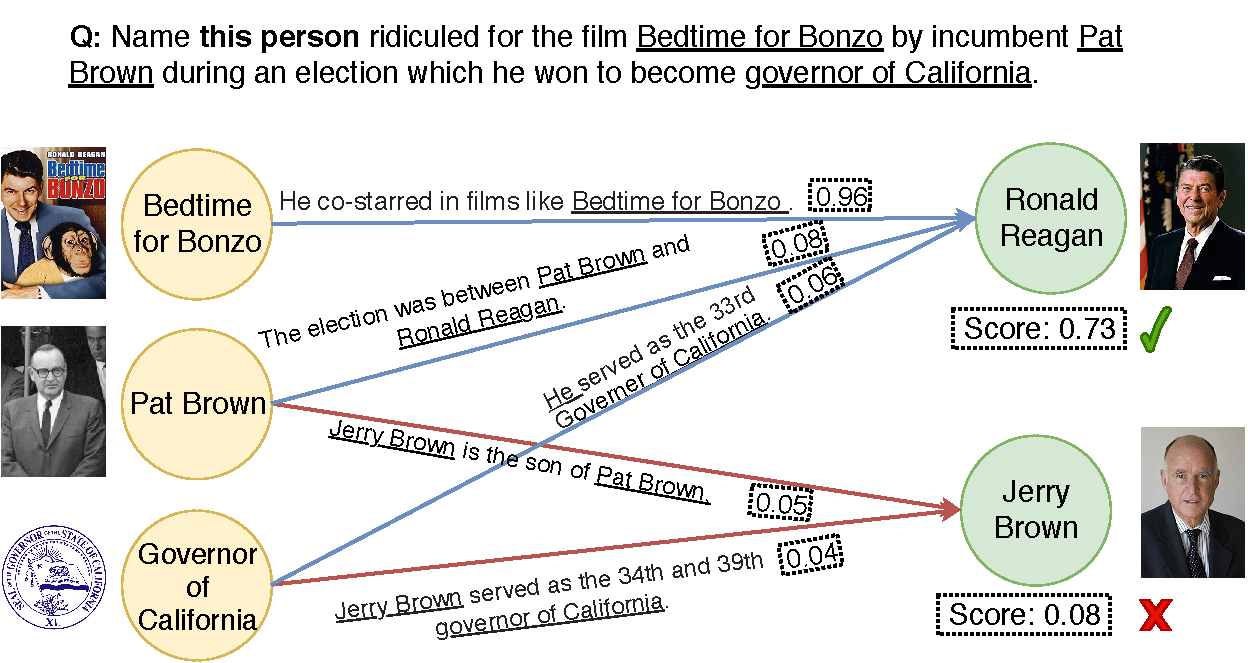
\includegraphics[width=0.9\linewidth]{2020_www_delft/figures/graph_vis_2020.pdf}
      \end{center}
      \caption{An example \name{} subgraph. The learned edge weights in \abr{gnn} are in the brackets. }
      \label{fig:graphvis}
\end{figure}



\paragraph{Model Ablation}

In addition to different data sources and preprocessing, \name{}
also has several model components.
%
We ablate these in Table~\ref{tab:ablation}.
%
As expected, both node (gloss) and edge evidence 
help; each contributes $\sim 10\%$ accuracy.
%
Edge importance scoring, which controls the weights of the information
flow from \leftnode{} to \rightnode{}s, provides $\sim 3\%$
accuracy.
%
The input representation is important as well; the self-attention
layer contributes $\sim 2.2\%$ accuracy.




\subsection{Graph Visualization}

Figure~\ref{fig:graphvis} shows a question with \abr{gnn} output:
%
the correct \rightnode{} \candidate{Ronald Reagan}
connects to all three \leftnode{}s.
%
The edge from \question{Bedtime for Benzo} to \candidate{Reagan} is
informative---other \rightnode{}s (e.g., politicians like
\candidate{Jerry Brown}) lack ties to this cinema masterpiece.
%
The \abr{gnn} model correctly (weight $0.96$) favors this edge.
%
The other edges are less distinguishable.
%
For example, the edge from \question{Governor of California} to
\candidate{Ronald Reagan} and \candidate{Jerry Brown} are both
relevant (both were governors) but unhelpful.
%
Thus, the \abr{gnn} has similar weights ($0.06$ and $0.04$) for
both edges, far less than \question{Bedtime for Bonzo}.
%
By aggregating edges, \name{}'s \abr{gnn} selects the correct
answer.


\subsection{Case Study}

To gain more insights into \name{} model's behavior, we further sample
some examples from \qblink{}.  Table~\ref{tab:example} shows two
positive examples ($1$ and $2$) and two negative examples ($3$ and
$4$).  \name{} succeeds on these cases: with direct evidence
sentences, \name{} finds the correct answer with high confidence
(Example 1) or with multiple pieces of evidence, \name{} could
aggregate different pieces together, and make more accurate
predictions (Example 2).  However some common sources of error
include: too few informative entities in the question (Example 3) or
evidence that overlaps too much between two \rightnode{}s.


%\paragraph{Direct Mapping}
%In example 1, direct evidence sentences are available, 
%\name{} finds the correct answer with high confidence. 
%\paragraph{Evidence Aggregation}
%Example 2 shows a more complicated question.  Since 
%the correct answer \candidate{Tom Brady} links to all essential question entities, \name{} 
%aggregates multiple piece of evidence from different question entities, 
%and \name{} makes the correct prediction. 
%Without the graph structure, \memnn{}  makes the wrong prediction \candidate{Stephon Gilmore}
% (Also a player from New England Patriots team).
%\paragraph{No Informative Entities}
%In example 3, \name{} makes a wrong prediction because there are no informative entities in the question. 
%The entity linker links can not infer ``western Germany'' 
%from \question{western regions}. Instead it links to entity
%``Xiyu''~\footnote{\url{https://en.wikipedia.org/wiki/Western_Regions}} 
%and leads to the wrong prediction ``Yumen Pass''.
%\paragraph{Wrong Reasoning}
%In example 4, even with the crucial evidence sentences, 
%%\name{} can not distinguish between 
%candidates \candidate{Odysseus} and \candidate{Penelope}.
%Since most evidence  applies to both candidates
%(e.g., their son \question{Telemachus}).






